\subsection{Introduction To Hadoop}

%%%%%%%%%%%%%%%%%%%%%%%%%%%%%%%%%%%%%%%%%%%%%%%%%%%%%%
\begin{frame}
	\frametitle{Lecture Objectives }
	\begin{itemize}  [<+->]
		\item Why do we need Hadoop?
		\item Hadoop Distributed File System (HDFS) concepts.
		\item Go dive into MapReduce.
		\item Hadoop architecture and its echosystems.
		\item How does Hadoop store, distribute, and process the data?

		
	\end{itemize}
\end{frame}
%%%%%%%%%%%%%%%%%%%%%%%%%%%%%%%%%%%%%%%%%%%%%%%%%%%%%%
\begin{frame}[c]{ }
	\frametitle{Introduction to Hadoop }
	\begin{itemize}  [<+->]
	\item Apache Hadoop's MapReduce and HDFS components were inspired by Google papers on MapReduce and Google File System
	
\end{itemize}
	\footnotetext[1]{From Wikipedia  \href{https://en.wikipedia.org/wiki/Apache_Hadoop}{https://en.wikipedia.org/wiki/Apache_Hadoop}	} 
	\footnotetext[2]{Google File System  \href{http://static.googleusercontent.com/media/research.google.com/en//archive/gfs-sosp2003.pdf}{http://static.googleusercontent.com/media/research.google.com/en//archive/gfs-sosp2003.pdf}	} 
	
	\footnotetext[3]{MapReduce: Simplifed Data Processing on Large Clusters \href{https://static.googleusercontent.com/media/research.google.com/en//archive/mapreduce-osdi04.pdf}{https://static.googleusercontent.com/media/research.google.com/en//archive/mapreduce-osdi04.pdf}	} 
	
\end{frame}

%%%%%%%%%%%%%%%%%%%%%%%%%%%%%%%%%%%%%%%%%%%%%%%%%%%%%%
\begin{frame}[c]{ }
		\frametitle{Introduction to Hadoop }
	\centering     
	
	\textcolor{offgreen}{ \large Is it already dead?}
\end{frame}
%%%%%%%%%%%%%%%%%%%%%%%%%%%%%%%%%%%%%%%%%%%%%%%%%%%%%%
\begin{frame}
	\frametitle{What is Hadoop? }
	\begin{itemize}  [<+->]
		\item A distributed software framework to store, process, and analzing "Large Scale of Data AKA. Big Data"
		\item It is open source!
		\item It runs on commodity (standard) hardware.
		\item Hadoop architecture and its echosystems.		
	\end{itemize}
\end{frame}
%%%%%%%%%%%%%%%%%%%%%%%%%%%%%%%%%%%%%%%%%%%%%%%%%%%%%%
\begin{frame}
	\frametitle{Hadoop Core Components }
	\begin{itemize}  [<+->]
		
		\item Hadoop HDFS: Data Storage Layer (File System).
		\item Hadoop MapReduce: The processing engine (compute paradigm) in Hadoop.
		\item Hadoop YARN: The resource manager in Hadoop.
		
	\end{itemize}
\end{frame}
%%%%%%%%%%%%%%%%%%%%%%%%%%%%%%%%%%%%%%%%%%%%%%%%%%%%%%
\begin{frame}[c]{ }
	\frametitle{Introduction to Hadoop }
	\centering     
	
	\textcolor{offgreen}{ \large What are the alternatives?}
\end{frame}
%%%%%%%%%%%%%%%%%%%%%%%%%%%%%%%%%%%%%%%%%%%%%%%%%%%%%%
\begin{frame}
	\frametitle{Hadoop Core Components }
	\begin{itemize}  
		
		\item \sout{Hadoop HDFS} \textcolor{offyellow}{S3/GFS}:  Data Storage Layer (File System).
		\item \sout{Hadoop MapReduce} \textcolor{offyellow}{Spark/Flink}: The processing engine (compute paradigm) in Hadoop.
		\item \sout{Hadoop YARN} \textcolor{offyellow}{Kubernetes}: The resource manager in Hadoop.
		% \textcolor{brown}{
	\end{itemize}
\end{frame}
%%%%%%%%%%%%%%%%%%%%%%%%%%%%%%%%%%%%%%%%%%%%%%%%%%%%%%
\begin{frame}[c]{ }
	\frametitle{Introduction to Hadoop }
	\centering     
	
	\textcolor{offgreen}{ \large Can we use these alternatives on prem?}
\end{frame}
%%%%%%%%%%%%%%%%%%%%%%%%%%%%%%%%%%%%%%%%%%%%%%%%%%%%%%
\begin{frame}
	\frametitle{Hadoop Echosystem }
	\begin{figure}
	\centering
	


\tikzset{every picture/.style={line width=0.75pt}} %set default line width to 0.75pt        


\def \xOne {12}
\def \xTwo {522}
\def \yOne {165}
\def \yTwo {195}
\def \yOneDelta {40}
\def \yTwoDelta {35}
\def \yTwoShift {5}

\def \hcboxXOne{20}
\def \hcboxXTwo{110}
\def \hcboxYOne{25}
\def \hcboxYTwo{50}
\def \hcboxXShift{100}

\def \dsXOne{60}
\def \dsXTwo{190}
\def \dsYOne{130}
\def \dsYTwo{155}
\def \dsXShift{270}

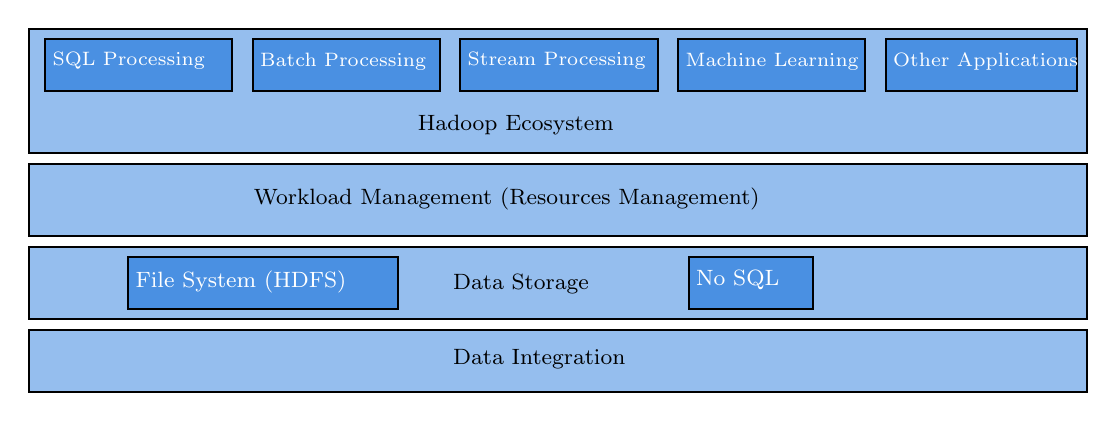
\begin{tikzpicture}[x=0.75pt,y=0.75pt,yscale=-1,xscale=1]

	
	%Shape: Rectangle [id:dp9526398227547324] 
	\draw [fill={rgb, 255:red, 74; green, 144; blue, 226 }  ,fill opacity=0.59 ] (\xOne,\yOne) -- (\xTwo,\yOne) -- (\xTwo,\yTwo) -- (\xOne,\yTwo) -- cycle ;
	%Shape: Rectangle [id:dp34591779607428674] 
	\draw  [fill={rgb, 255:red, 74; green, 144; blue, 226 }  ,fill opacity=0.59 ] (\xOne,\yOne-\yOneDelta) -- (\xTwo,\yOne-\yOneDelta) -- (\xTwo,\yTwo-\yTwoDelta) -- (\xOne,\yTwo-\yTwoDelta) -- cycle ;

	%Shape: Rectangle [id:dp45758690857887285] 
	\draw [fill={rgb, 255:red, 74; green, 144; blue, 226 }  ,fill opacity=0.59 ] (\xOne,\yOne-\yOneDelta*2) -- (\xTwo,\yOne-\yOneDelta*2) -- (\xTwo,\yTwo-\yTwoDelta*2 - \yTwoShift) -- (\xOne,\yTwo-\yTwoDelta*2 - \yTwoShift) -- cycle ;
	%Shape: Rectangle [id:dp7537784714823494] 
	\draw [fill={rgb, 255:red, 74; green, 144; blue, 226 }  ,fill opacity=0.59 ] (\xOne,\yOne-\yOneDelta*3-25) -- (\xTwo,\yOne-\yOneDelta*3-25) -- (\xTwo,\yTwo-\yTwoDelta*3 -\yTwoShift*2) -- (\xOne,\yTwo-\yTwoDelta*3 -\yTwoShift*2) -- cycle ;
	
	
	%Rounded Rect [id:dp9146242593539052] 
	\draw  [fill={rgb, 255:red, 74; green, 144; blue, 226 }  ,fill opacity=1 ] (\dsXOne,\dsYOne) -- (\dsXTwo,\dsYOne) -- (\dsXTwo,\dsYTwo) -- (\dsXOne,\dsYTwo) -- cycle ;
	%Rounded Rect [id:dp07383423201361416] 
	\draw  [fill={rgb, 255:red, 74; green, 144; blue, 226 }  ,fill opacity=1 ] (\dsXOne+\dsXShift,\dsYOne) -- (\dsXTwo-70+\dsXShift,\dsYOne) -- (\dsXTwo+\dsXShift-70,\dsYTwo) -- (\dsXOne+\dsXShift,\dsYTwo) -- cycle ;
	
	
	
	
	%Rounded Rect [id:dp8181874793090042] 
	\draw  [fill={rgb, 255:red, 74; green, 144; blue, 226 }  ,fill opacity=1 ] (\hcboxXOne,\hcboxYOne) -- (\hcboxXTwo,\hcboxYOne) -- (\hcboxXTwo,\hcboxYTwo) -- (\hcboxXOne,\hcboxYTwo) -- cycle ;
	%Rounded Rect [id:dp9716087561496145] 
	\draw  [fill={rgb, 255:red, 74; green, 144; blue, 226 }  ,fill opacity=1 ] (\hcboxXOne+\hcboxXShift,\hcboxYOne) -- (\hcboxXTwo+\hcboxXShift,\hcboxYOne) -- (\hcboxXTwo+\hcboxXShift,\hcboxYTwo) -- (\hcboxXOne+\hcboxXShift,\hcboxYTwo) -- cycle ;
	%Rounded Rect [id:dp6064393858129398] 
	\draw  [fill={rgb, 255:red, 74; green, 144; blue, 226 }  ,fill opacity=1 ] (\hcboxXOne+\hcboxXShift*2,\hcboxYOne) -- (\hcboxXTwo+\hcboxXShift*2+5,\hcboxYOne) -- (\hcboxXTwo+\hcboxXShift*2+5,\hcboxYTwo) -- (\hcboxXOne+\hcboxXShift*2,\hcboxYTwo) -- cycle ;
	%Rounded Rect [id:dp9339323209047331] 
	\draw  [fill={rgb, 255:red, 74; green, 144; blue, 226 }  ,fill opacity=1 ] (\hcboxXOne+\hcboxXShift*3+5,\hcboxYOne) -- (\hcboxXTwo+\hcboxXShift*3+5,\hcboxYOne) -- (\hcboxXTwo+\hcboxXShift*3+5,\hcboxYTwo) -- (\hcboxXOne+\hcboxXShift*3+5,\hcboxYTwo) -- cycle ;
	%Rounded Rect [id:dp5657335982682512] 
	\draw  [fill={rgb, 255:red, 74; green, 144; blue, 226 }  ,fill opacity=1 ] (\hcboxXOne+\hcboxXShift*4+5,\hcboxYOne) -- (\hcboxXTwo+\hcboxXShift*4+7,\hcboxYOne) -- (\hcboxXTwo+\hcboxXShift*4+7,\hcboxYTwo) -- (\hcboxXOne+\hcboxXShift*4+5,\hcboxYTwo) -- cycle ;

	% Text Node
	\draw (215,173) node [anchor=north west][inner sep=0.75pt]  [font=\footnotesize] [align=left] {Data Integration};
	% Text Node
	\draw (\dsXOne+2,\dsYOne+5) node [anchor=north west][inner sep=0.75pt]  [font=\footnotesize,color={rgb, 255:red, 255; green, 255; blue, 255 }  ,opacity=1 ] [align=left] {File System (HDFS)};
	% Text Node
	\draw (\dsXOne+\dsXShift+2,\dsYOne+5) node [anchor=north west][inner sep=0.75pt]  [font=\footnotesize,color={rgb, 255:red, 255; green, 255; blue, 255 }  ,opacity=1 ] [align=left] {No SQL};

	% Text Node
	\draw (215,137) node [anchor=north west][inner sep=0.75pt]  [font=\footnotesize] [align=left] {Data Storage};
	% Text Node
	\draw (119,95) node [anchor=north west][inner sep=0.75pt]  [font=\footnotesize] [align=left] {Workload Management (Resources Management)};
	% Text Node
	\draw (198,60) node [anchor=north west][inner sep=0.75pt]  [font=\footnotesize] [align=left] {Hadoop Ecosystem};
	
	% Text Node
	\draw (\hcboxXOne +2 ,\hcboxYOne +5) node [anchor=north west][inner sep=0.75pt]  [font={\scriptsize },color={rgb, 255:red, 255; green, 255; blue, 255 }  ,opacity=1 ] [align=left] {SQL Processing};
	% Text Node
	\draw (\hcboxXOne +2+\hcboxXShift,\hcboxYOne +5) node [anchor=north west][inner sep=0.75pt]  [font=\scriptsize,color={rgb, 255:red, 255; green, 255; blue, 255 }  ,opacity=1 ] [align=left] {Batch Processing};
	% Text Node
	\draw (\hcboxXOne +2+\hcboxXShift*2,\hcboxYOne +5) node [anchor=north west][inner sep=0.75pt]  [font=\scriptsize,color={rgb, 255:red, 255; green, 255; blue, 255 }  ,opacity=1 ] [align=left] {Stream Processing};
	% Text Node
	\draw (\hcboxXOne +7+\hcboxXShift*3,\hcboxYOne +5) node [anchor=north west][inner sep=0.75pt]  [font=\scriptsize,color={rgb, 255:red, 255; green, 255; blue, 255 }  ,opacity=1 ] [align=left] {Machine Learning};
	% Text Node
	\draw (\hcboxXOne +7+\hcboxXShift*4,\hcboxYOne +5) node [anchor=north west][inner sep=0.75pt]  [font=\scriptsize,color={rgb, 255:red, 255; green, 255; blue, 255 }  ,opacity=1 ] [align=left] {Other Applications};
	
	
\end{tikzpicture}
%%%%%%%%%%%%%%%%%%%%%%%%%%%%%%%%%%%%%%%%%%%%%%%%%%%%%%%%%%%%%%%%%%%%%%%%%%%
%%% Local Variables:
%%% mode: latex
%%% TeX-master: "../../main.tex"
% !TeX root = ../../main.tex
%%% TeX-engine: xetex
%%% End:

	\caption{Hadoop Architecture } \label{fig:DS3}
\end{figure}
\end{frame}
%%%%%%%%%%%%%%%%%%%%%%%%%%%%%%%%%%%%%%%%%%%%%%%%%%%%%%
\begin{frame}[c]{ }
	\frametitle{Hadoop Motivation }
	\centering     
	
	\textcolor{offgreen}{ \large Hadoop Motivation}
\end{frame}
%%%%%%%%%%%%%%%%%%%%%%%%%%%%%%%%%%%%%%%%%%%%%%%%%%%%%%
\begin{frame}[c]{ }
	\frametitle{Hadoop Motivation }
	Processing:
	\begin{itemize}  [<+->]
	
	\item Traditional Computation was depending on bigger computers to deal with bigger data.
	\item This method has a bottleneck in the computation (Moore's Law), but this couldn't keep up.
	\item The better solution requires more computers (distributed computing framework).
	
\end{itemize}
\end{frame}
%%%%%%%%%%%%%%%%%%%%%%%%%%%%%%%%%%%%%%%%%%%%%%%%%%%%%%
\begin{frame}[c]{ }
	\frametitle{Hadoop Motivation }
	Storage:
	\begin{itemize}  [<+->]
		
		\item Traditional Computation store the data in a central unit.
		\item Data was copied (moved) to the computation nodes, for example, IBM Data stage or Talend.
		\item The process of copying or moving the data was fine when we move a small amount of data, but the big data will cause lots of problems, especially in the network bandwidth, and data moving will be costly.
		
	\end{itemize}
\end{frame}

%%%%%%%%%%%%%%%%%%%%%%%%%%%%%%%%%%%%%%%%%%%%%%%%%%%%%%
\begin{frame}[c]{ }
	\frametitle{Requirements for The New Approach }
	
	
	\begin{itemize}  [<+->]
		\item [--] Fault Tolerance.
		\item [--] High Availability.
		\item [--] Reliability.
		\item [--] Scalability.
		\item [--] Consistency.
		\item [--] Data Locality.
		\item [--] Economic.
		
	\end{itemize}
\end{frame}
%%%%%%%%%%%%%%%%%%%%%%%%%%%%%%%%%%%%%%%%%%%%%%%%%%%%%%
\begin{frame}[c]{ }
	\frametitle{Requirements for The New Approach }
	Economic
	\begin{itemize}  [<+->]
		\item [--] {\footnotesize It uses commodity (Standard/Economic) hardware}.

	\end{itemize}
\end{frame}
%%%%%%%%%%%%%%%%%%%%%%%%%%%%%%%%%%%%%%%%%%%%%%%%%%%%%%
\begin{frame}[c]{ }
	\frametitle{Requirements for The New Approach }
	Data Locality
	\begin{itemize}  [<+->]
		\item [--] {\footnotesize It brings the program to the data rather than the data to the program. It runs the computation where the data reside.}		
		\item [--] {\footnotesize HDFS is strongly consistent.}		
	\end{itemize}
\end{frame}
%%%%%%%%%%%%%%%%%%%%%%%%%%%%%%%%%%%%%%%%%%%%%%%%%%%%%%
\begin{frame}[c]{ }
	\frametitle{Requirements for The New Approach }
	Fault Tolerance
	\begin{itemize}  [<+->]
		\item [--] {\footnotesize It is the property that enables a system to continue operating properly in the event of the failure of (or one or more faults within) some of its components}.
		\item [--] {\footnotesize The ability of maintaining functionality when portions of a system break down is referred to as graceful degradation}.
		\item [--] {\footnotesize A fault-tolerant design enables a system to continue its intended operation, possibly at a reduced level, rather than failing completely, when some part of the system fails.}
		
	\end{itemize}
	\footnotetext[1]{From Wikipedia  \href{https://en.wikipedia.org/wiki/Fault_tolerance}{https://en.wikipedia.org/wiki/Fault_tolerance}	} 
\end{frame}
%%%%%%%%%%%%%%%%%%%%%%%%%%%%%%%%%%%%%%%%%%%%%%%%%%%%%%
\begin{frame}[c]{ }
	\frametitle{Requirements for The New Approach }
	High Availability
	\begin{itemize}  [<+->]
		\item [--] {\footnotesize High availability (HA) is a characteristic of a system which aims to ensure an agreed level of operational performance, usually uptime, for a higher than normal period}.
		\item [--] {\footnotesize The availability of the cluster (system) to operate without any downtime despite any hardware failure. The data or the system should be available and accessed from any alternative way}.
		
	\end{itemize}
	\footnotetext[1]{From Wikipedia  \href{https://en.wikipedia.org/wiki/High_availability}{https://en.wikipedia.org/wiki/High_availability}	} 
\end{frame}

%%%%%%%%%%%%%%%%%%%%%%%%%%%%%%%%%%%%%%%%%%%%%%%%%%%%%%
\begin{frame}[c]{ }
	\frametitle{Requirements for The New Approach }
	Reliability
	\begin{itemize}  [<+->]
		\item [--] {\footnotesize The data reliably stored on the cluster of machine despite machine failures. }		
	\end{itemize}
\end{frame}
%%%%%%%%%%%%%%%%%%%%%%%%%%%%%%%%%%%%%%%%%%%%%%%%%%%%%%
\begin{frame}[c]{ }
	\frametitle{Requirements for The New Approach }
	Scalability
	\begin{itemize}  [<+->]
		\item [--] {\footnotesize The system must be highly scalable in both vertical and horizontal. This means we can add a new node to an existing cluster easily or add new hardware to an existing node.}		
	\end{itemize}
\end{frame}
%%%%%%%%%%%%%%%%%%%%%%%%%%%%%%%%%%%%%%%%%%%%%%%%%%%%%%
\begin{frame}[c]{ }
	\frametitle{Requirements for The New Approach }
	Consistency
	\begin{itemize}  [<+->]
		\item [--] {\footnotesize Any failure during the execution job shouldn't affect the outcome of the job.}		
		\item [--] {\footnotesize HDFS is strongly consistent.}		
	\end{itemize}
\end{frame}
%%%%%%%%%%%%%%%%%%%%%%%%%%%%%%%%%%%%%%%%%%%%%%%%%%%%%%
\begin{frame}[c]{ }
	\frametitle{Core Hadoop Concepts }
	\centering     
	
	\textcolor{offgreen}{ \large Hadoop Core Concepts}
\end{frame}
%%%%%%%%%%%%%%%%%%%%%%%%%%%%%%%%%%%%%%%%%%%%%%%%%%%%%%
\begin{frame}[c]{ }
	\frametitle{Hadoop Core Concepts }
	
	
	\begin{itemize}  [<+->]
		\item [--] Hadoop is scalable and fault-tolerant.
		\item [--] Hadoop replicates the data to increase the availability and reliability.
		\item [--] Hadoop brings the program to the data.
		\item [--] Applications are written in high-level code.
		\item [--] Hadoop reduces the data movement (shuffle) between the nodes.
		
	\end{itemize}
\end{frame}
